
\begin{figure*}[h!]%
 \centering
 \subfloat[BRISK]{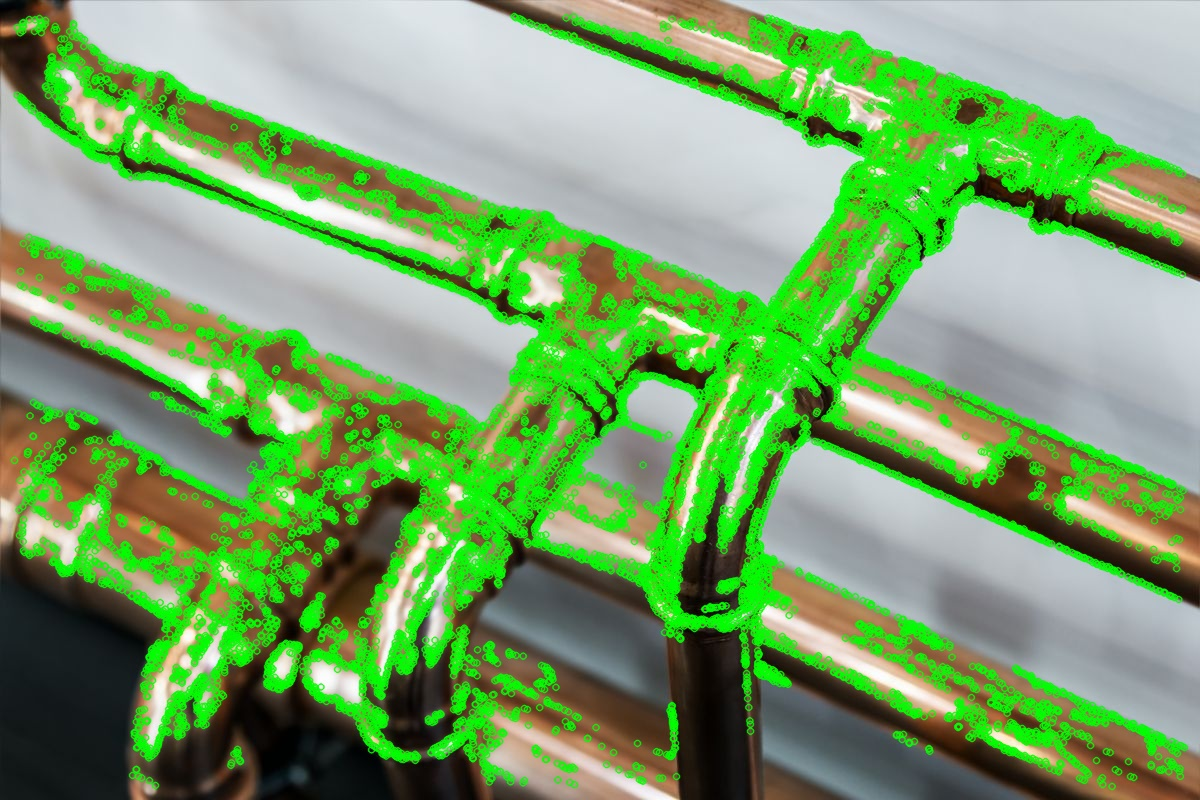
\includegraphics[width=\textwidth/2]{images/BRISK.jpg}\label{fig:a}}\hspace*{3em}%
 \subfloat[SURF]{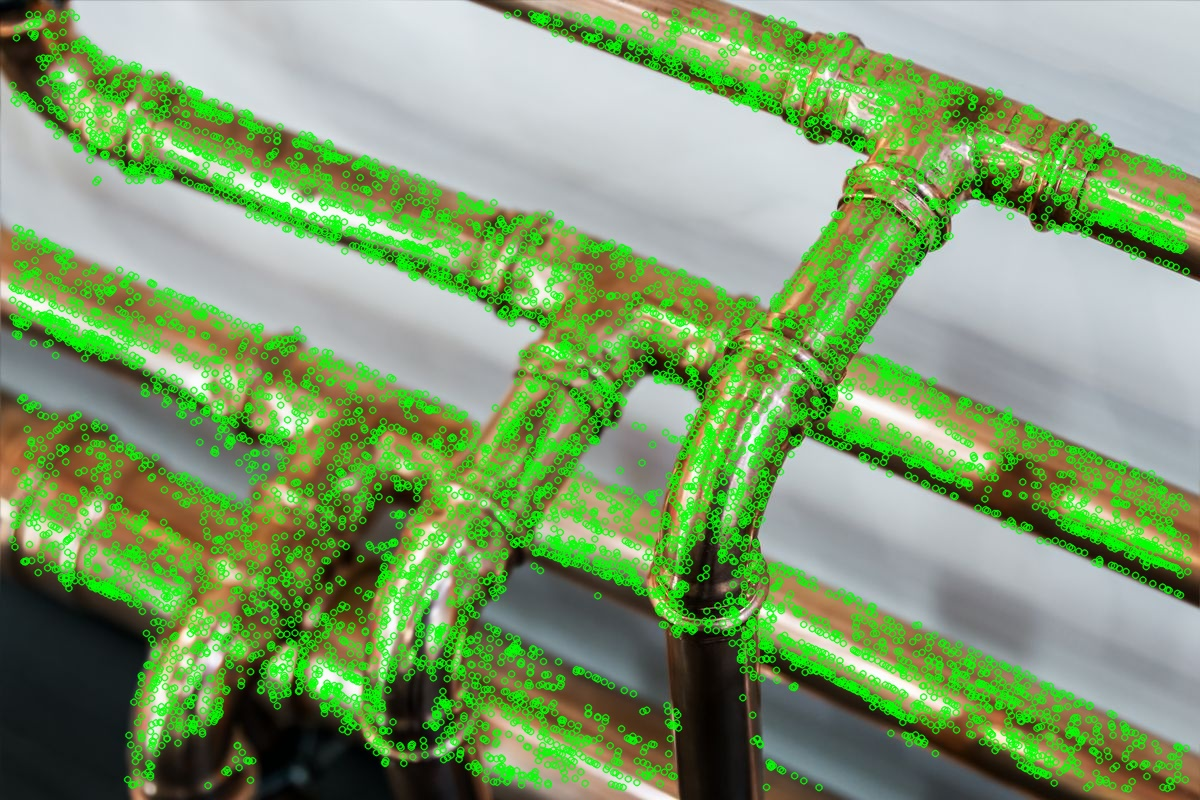
\includegraphics[width=\textwidth/2]{images/SURF.jpg}\label{fig:b}}\\
 \subfloat[BRISK overlaid on Superpixel]{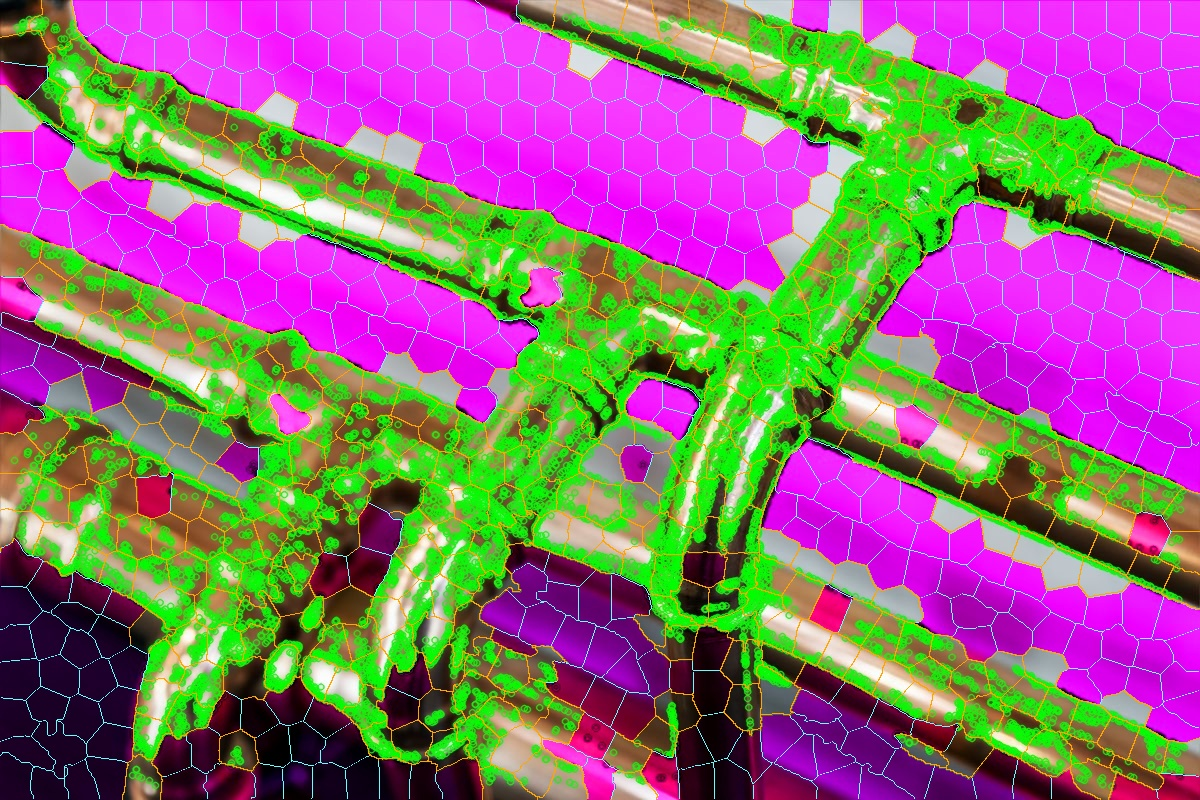
\includegraphics[width=\textwidth/2]{images/superpixel.jpg}\label{fig:c}}\hspace*{3em}%
 \subfloat[Colormap Channel-Reduction]{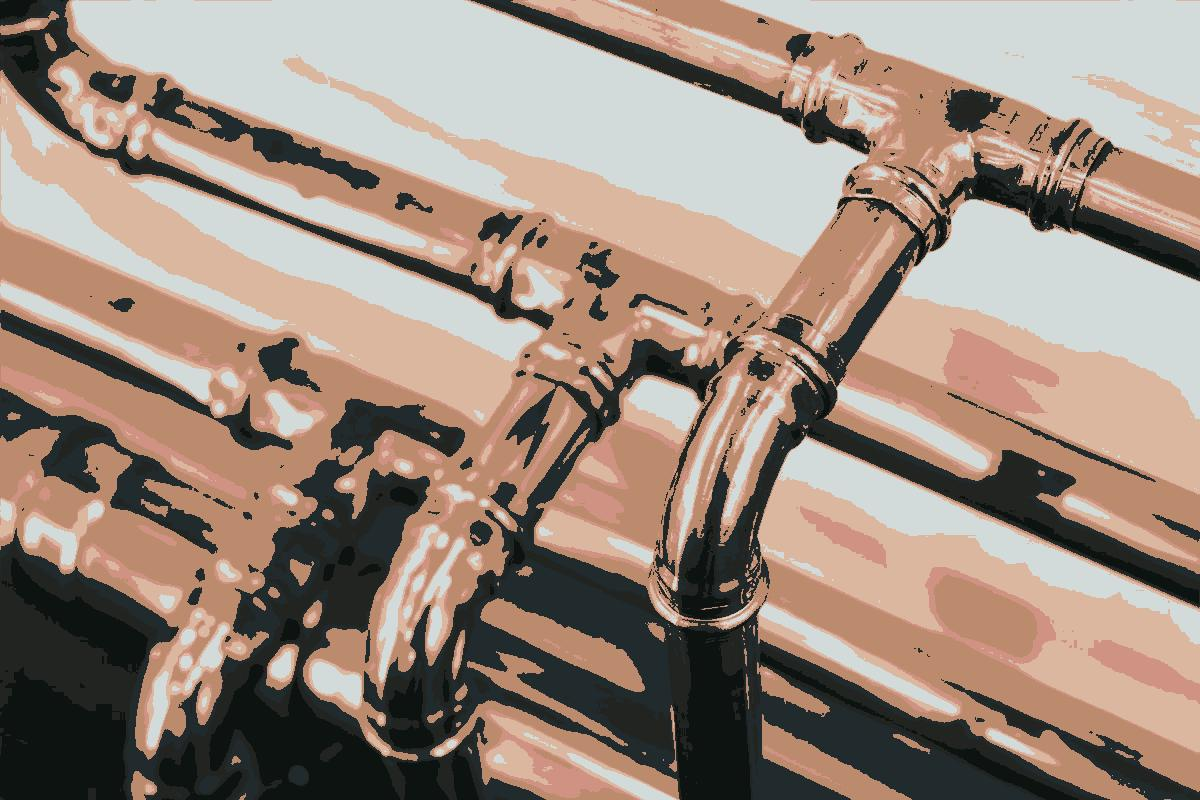
\includegraphics[width=\textwidth/2]{images/eight.jpg}\label{fig:d}}\\%
 \caption{Localizing Keypoints to the Image-Foreground}%
 \label{fig:all}%
{\labelbox{Two keypoint detectors yielding good results for this 
workflow, BRISK (Binary Robust Invariant Scalable Keypoints) 
and SURF (Speeded Up Robust Features) [a, b].  Combined 
with a superpixel segmentation, the foreground could be  
detected by extending the feature point-cloud to 
the set of superpixels containing one keypoint (or some count 
of keypoints, beyond a chosen threshold) [c].  
This superpixel segmentation uses a different 
channel-reduction via mapping the full set of 
image-pixels onto a small collection of the 
most frequent colors, according to toroidal distance [d].}} 
\end{figure*}


